% Find documentation here:
% - https://ctan.org/pkg/tudscr?lang=en
% - https://github.com/tud-cd/tudscr/blob/main/source/doc/examples/poster.tex

\RequirePackage{fix-cm}
\documentclass[%
  english,%
  paper=A1,%
  fontsize=22pt,%
  cdfoot=5ex,%
  ddcfoot,%
  %shift text format field left and right
  BCOR=-20mm,
]{tudscrposter}

\usepackage[T1]{fontenc}
\usepackage{babel}
\usepackage{import}
\usepackage{blindtext}
\usepackage{multicol}
\usepackage{tabularx}
\usepackage{qrcode}
\usepackage{graphicx}
\usepackage{tikz}
\usetikzlibrary{backgrounds}
\usepackage{svg}
\usepackage{pdfpages}
\usepackage{wrapfig}
\usepackage{xcolor}
\usepackage{tcolorbox} % farbige Boxen


\definecolor{messagespace}{HTML}{e6c6d9}
\definecolor{messageselection}{HTML}{9bcff2}
\definecolor{encoding}{HTML}{73c2aa}
\definecolor{tagextraction}{HTML}{f0c985}
\definecolor{tagcomparison}{HTML}{f6ee91}


% --- Math Packages ---
\usepackage{amsmath}        % Advanced math environments
\usepackage{amssymb}        % Extra math symbols
\usepackage{mathtools}      % Further math tools, loads amsmath
\usepackage{commath}        % For common math commands like \dif
\usepackage{amsthm}         % For theorem and proof environments


\usepackage[acronym]{glossaries} % 
\newacronym{tsn}{TSN}{Time-Sensitive Networking}
\newacronym{fifo}{FIFO}{First-In-First-Out}
\newacronym{qos}{QoS}{Quality-of-Service}
\newacronym{tas}{TAS}{Time-aware Shaper}
\newacronym{spq}{SPQ}{Strict Priority Queuing}
\newacronym{af}{AF}{Application Function}
\newacronym{upf}{UPF}{User Plane Function}
\newacronym{tt}{TT}{TSN Translator}
\newacronym{dstt}{DS-TT}{Device-Side TSN Translator}
\newacronym{nwtt}{NW-TT}{Network-Side TSN Translator}
\newacronym{gui}{GUI}{Graphical User Interface}
\newacronym{sdr}{SDR}{Software-defined Radio}
\newacronym{ue}{UE}{User Equipment}
\newacronym{cots}{COTS}{Commercial-off-the-Shelf}
\newacronym{ptp}{PTP}{Precision Time Protocol}
\newacronym{ran}{RAN}{Radio Access Network}
\newacronym{TI}{TI}{Tactile Internet}

\begin{document}
\newcommand{\rarrow}{$\rightarrow$ }

%Mathematische Notation der gängigen Mengen
\newcommand{\RR}{\mathbb{R}} %reelle Zahlen
\newcommand{\CC}{\mathbb{C}} %komplexe Zahlen
\newcommand{\QQ}{\mathbb{Q}}
\newcommand{\NN}{\mathbb{N}}
\newcommand{\ZZ}{\mathbb{Z}}
\newcommand{\Prob}{\mathbb{P}} % Wahrscheinlichkeit

\newcommand{\gerquote}[1]{\glqq #1\grqq} %Deutsche Version der Anführungszeichen

% \newdateformat{myformat}{\THEDAY{ten }\monthnamengerman[\THEMONTH], \THEYEAR}
\headlogo{figures/ComNets_MZ_NEG_Subline_en.eps}

\faculty{Faculty of Electrical and Computer Engineering}
\department[]{}
\institute{Institute of Communication Technology}
\chair[]{}
\title{Identification System Evaluation \hfill }
\subtitle{\small Hauptseminar Kommunikationssysteme 2025}
\date{}
\contactperson{}
\professor{}
 
\footcontent{
    \hspace{-5cm}
    \begin{minipage}{5cm}
        \centering
        \qrcode[height=5cm]{https://idsystem.streamlit.app}\\[0.5em]
        \small ID Systems Dashboard
    \end{minipage}
    \hspace{2cm}
    \begin{tabularx}{0.85\textwidth}{X l}
        &\textbf{Authors}\\
        \textbf{Technische Universität Dresden}          \hfill & Antonio Döring\\
        Faculty of Electrical and Computer Engineering   \hfill & Armin Jacobi von Wangelin\\
        Institute of Communication Technology            \hfill & Nick Schubert\\
        Deutsche Telekom Chair of Communication Networks \hfill & Caroline Weisser\\
        Prof. Dr.-Ing. Dr. h.c. Frank H.P. Fitzek        \hfill & \textbf{Supervisor}\\
        &M. Sc. Caspar v. Lengerke
    \end{tabularx}
}

\maketitle
%\noindent by Antonio Döring, Armin Jacobi von Wangelin, Nick Schubert and Caroline Weisser
\setlength\parindent{0pt}
%\begin{abstract}[columns=3]
\begin{multicols}{3}
The project comprises a systematic evaluation of noiseless identification (ID) systems with a focus on ID tagging codes. Within the scope of goal-oriented communication, identification wants to determine whether  selected messages at the sender and receiver are identical. ID codes are designed to enable the transmission of reduced information, thereby decreasing bandwidth consumption. Nevertheless, this evokes possible errors in the verification step.\\
In the project, a modular test framework analyzes various ID coding schemes across different parameters and key metrics are visualized in an interactive dashboard.
Additional scenarios, including k-Identification and multiple tag transmission, are investigated to assess their impact on system reliability and computational overhead.
Furthermore, the behavior of ID codes under non-uniform message distributions is analyzed, revealing that certain encoders effectively randomize structured inputs, whereas others exhibit notable weaknesses in these cases.\\
The results highlight trade-offs between reliability, computational complexity and code rate in the design of practical ID systems. They can be viewed on the dashboard via the QR code in the bottom left corner.
\end{multicols}
%\end{abstract}
\vspace{1cm}

\hspace{-2.3cm}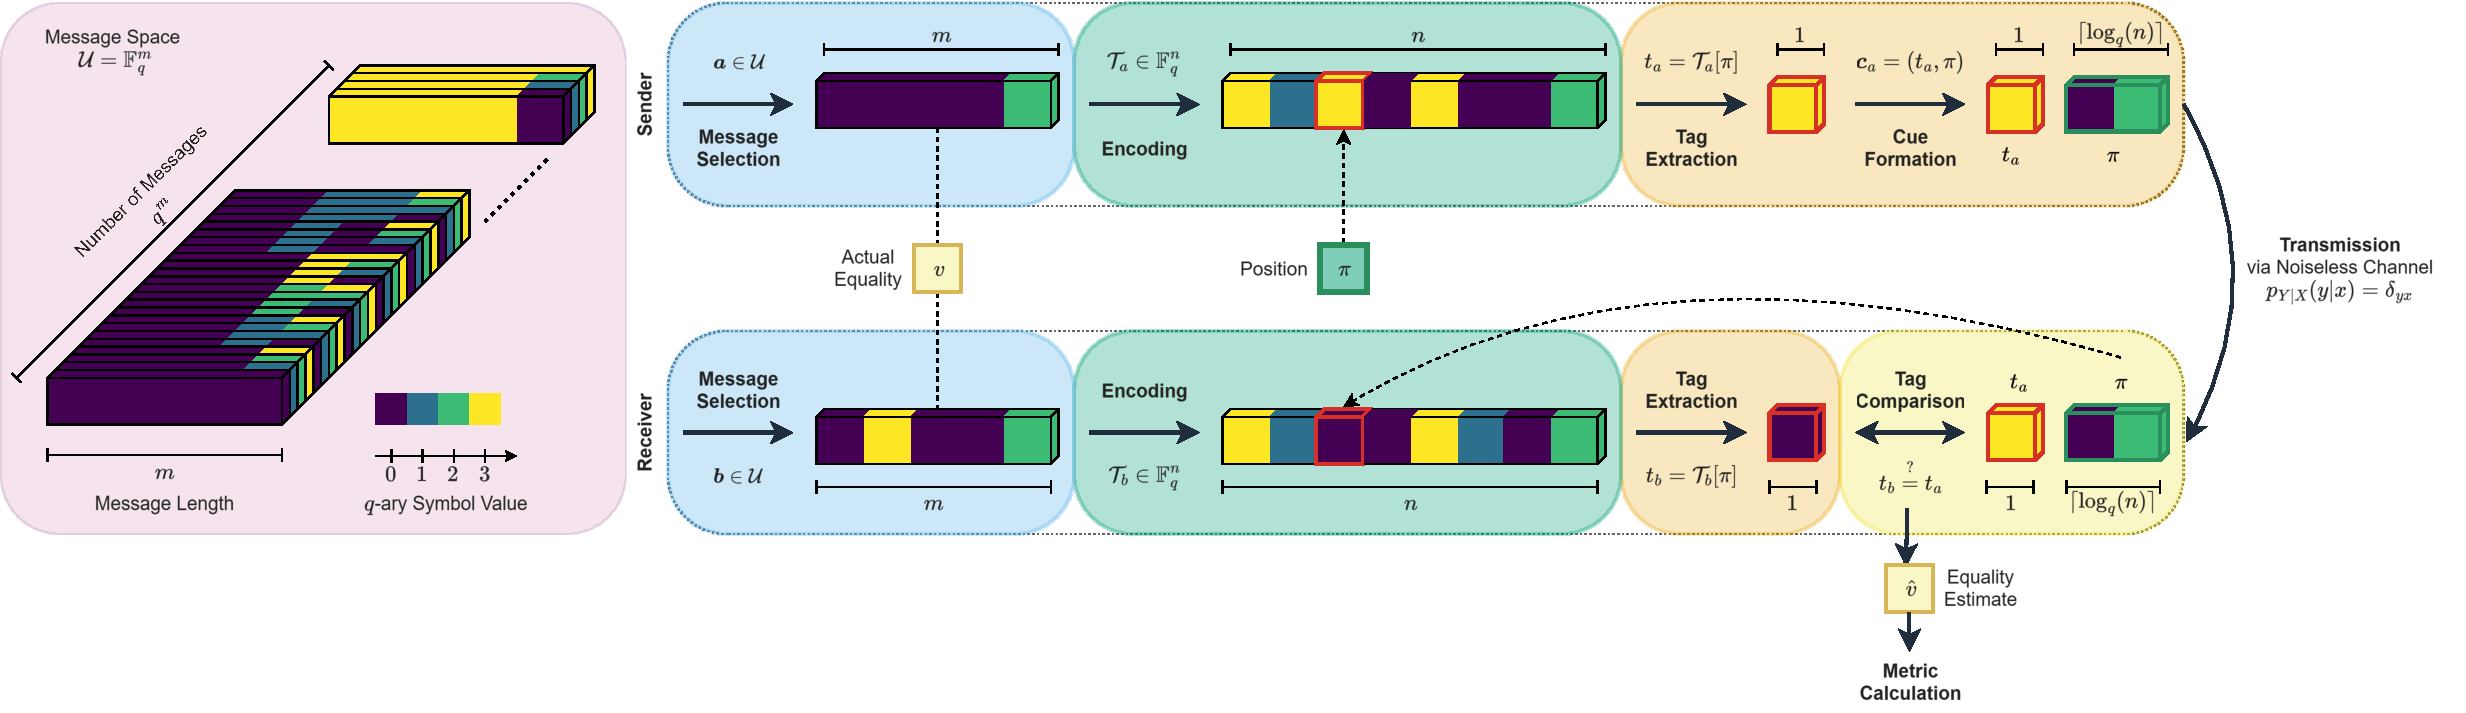
\includegraphics[width = 1.1\textwidth]{figures/ID_flow-Main Graph.drawio.pdf}

\begin{multicols}{3}%[\section*{Section Title}]

\begin{tcolorbox}[colback=messagespace!30, colframe=messagespace, boxrule=0pt, left=0pt, right=0pt, top=2pt, bottom=2pt, enlarge left by=-\marginparsep, width=.33\textwidth]
\subsubsection*{Message Space}
\end{tcolorbox}

\vspace{-0.2cm}

Sender and receiver share a common set of messages with the length $m$. There are $q^m$ different ways to generate the messages.


\vspace{0.5cm}

\begin{tcolorbox}[colback=messageselection!30, colframe=messageselection, boxrule=0pt, left=0pt, right=0pt, top=2pt, bottom=2pt, enlarge left by=-\marginparsep, width=.33\textwidth]
\subsubsection*{Message Selection}
\end{tcolorbox}

\vspace{-0.2cm}

The sender selects the message it wants to communicate with the receiver. Similarly, the receiver chooses a message it guesses the sender wants to send.


\vspace{0.5cm}

\begin{tcolorbox}[colback=encoding!30, colframe=encoding, boxrule=0pt, left=0pt, right=0pt, top=2pt, bottom=2pt, enlarge left by=-\marginparsep, width=.33\textwidth]
\subsubsection*{Encoding}
\end{tcolorbox}

\vspace{-0.2cm}

In the first step, the message is encoded, e.g., with an FEC code to increase the Hamming distance or a hash function. 

\vspace{0.5cm}

\begin{tcolorbox}[colback=tagextraction!30, colframe=tagextraction, boxrule=0pt, left=0pt, right=0pt, top=2pt, bottom=2pt, enlarge left by=-\marginparsep, width=.33\textwidth]
\subsubsection*{Tag Extraction and Cue Formation}
\end{tcolorbox}

\vspace{-0.2cm}

Afterwards, one symbol (tag) is extracted and together with its position in the encoded message, it forms the cue.

\vspace{0.5cm}

\begin{tcolorbox}[colback=tagcomparison!30, colframe=tagcomparison, boxrule=0pt, left=0pt, right=0pt, top=2pt, bottom=2pt, enlarge left by=-\marginparsep, width=.33\textwidth]
\subsubsection*{Transmission and Tag Comparison}
\end{tcolorbox}

\vspace{-0.2cm}

The cue is transmitted via an assumed noiseless channel. The receiver finally compares the received to its own tag for equality. This bit is used to calculate the metrics.
\columnbreak

\subsubsection*{Message Patterns}
\begin{wrapfigure}{r}{.16\textwidth}
    \centering
    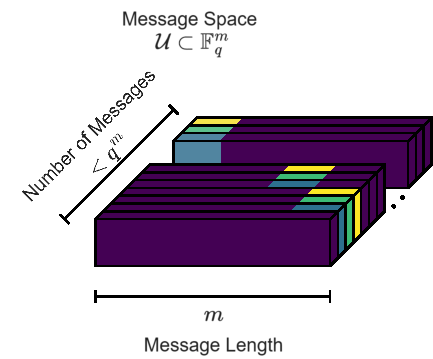
\includegraphics{figures/ID_flow-Message Patterns.pdf}
\end{wrapfigure}
Not in any case, the whole message space is used. The encoding process should be able to convert a narrow message distribution to a uniform tag distribution since this is beneficial with regard to system reliability. Reed-Solomon encoding performs very well whereas Reed-Muller does not achieve this objective.

\subsubsection*{k-Identification}
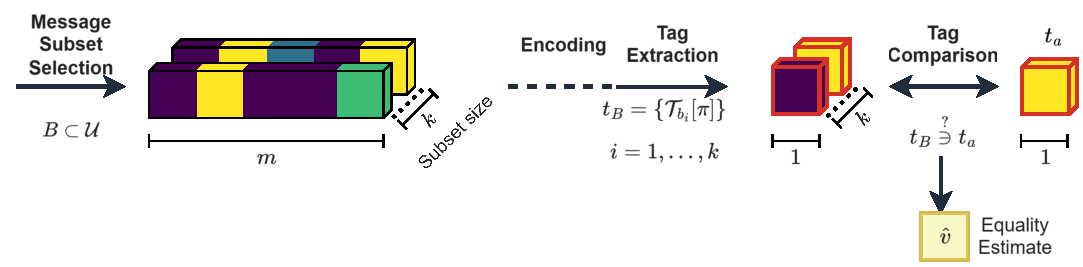
\includegraphics[width=0.32\textwidth]{figures/ID_flow-k-ID.drawio.pdf}
In the scenario of k-Identification, the receiver groups messages into subsets and tries to determine whether the received tag matches to at least one of the tags in the selected subset. This gives the system a certain tolerance, which is expressed in an increased success probability $ \mathbb{P}(\boldsymbol{a} \in B)$. However, the error probability is increased if the right message is not in the subset. For this reason, an appropriate partitioning of messages into subsets is crucial for the use of this scenario.

\subsubsection*{Multiple Tag Transmission}
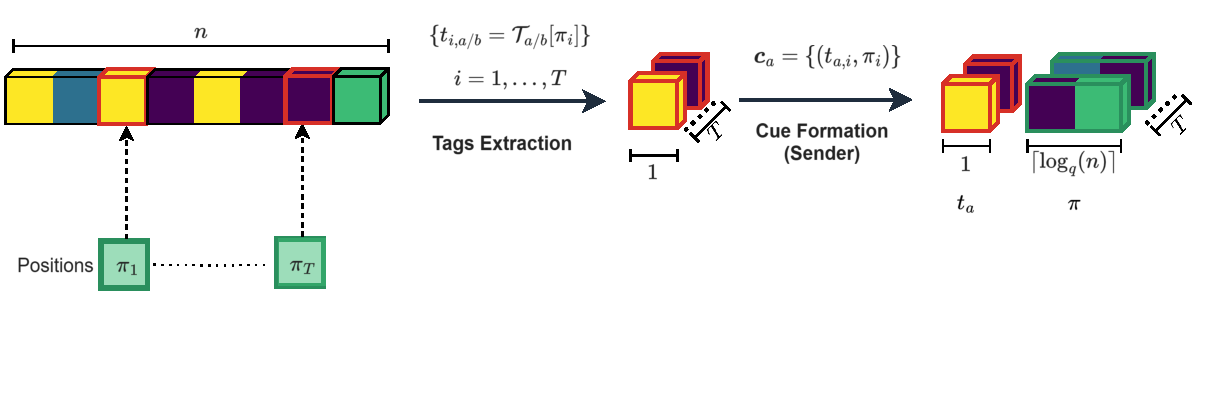
\includegraphics[width=0.32\textwidth]{figures/ID_flow-Multitag.drawio.pdf}
An approach to improve the system reliability is the transmission of multiple tags. This exponentially decreases the error probability while decreasing the code rate as well. To address this problem, we propose a protocol of subsequent tag transmission. In this way, the following tag is only transmitted if the previous all yielded a positive equality estimate, which reduces the average number of tags by the cost of a feedback channel and additional processing.


% \subsubsection*{Framework and Dashboard}
% The framework takes a system and parameter description. It creates messages and inserts them into the ID system. The equality estimate then is evaluated and the output metrics are visualized in the dashboard. 

\end{multicols}



\end{document}
